% Options for packages loaded elsewhere
\PassOptionsToPackage{unicode}{hyperref}
\PassOptionsToPackage{hyphens}{url}
\PassOptionsToPackage{dvipsnames,svgnames,x11names}{xcolor}
%
\documentclass[
  letterpaper,
  DIV=11,
  numbers=noendperiod]{scrartcl}

\usepackage{amsmath,amssymb}
\usepackage{iftex}
\ifPDFTeX
  \usepackage[T1]{fontenc}
  \usepackage[utf8]{inputenc}
  \usepackage{textcomp} % provide euro and other symbols
\else % if luatex or xetex
  \usepackage{unicode-math}
  \defaultfontfeatures{Scale=MatchLowercase}
  \defaultfontfeatures[\rmfamily]{Ligatures=TeX,Scale=1}
\fi
\usepackage{lmodern}
\ifPDFTeX\else  
    % xetex/luatex font selection
\fi
% Use upquote if available, for straight quotes in verbatim environments
\IfFileExists{upquote.sty}{\usepackage{upquote}}{}
\IfFileExists{microtype.sty}{% use microtype if available
  \usepackage[]{microtype}
  \UseMicrotypeSet[protrusion]{basicmath} % disable protrusion for tt fonts
}{}
\makeatletter
\@ifundefined{KOMAClassName}{% if non-KOMA class
  \IfFileExists{parskip.sty}{%
    \usepackage{parskip}
  }{% else
    \setlength{\parindent}{0pt}
    \setlength{\parskip}{6pt plus 2pt minus 1pt}}
}{% if KOMA class
  \KOMAoptions{parskip=half}}
\makeatother
\usepackage{xcolor}
\setlength{\emergencystretch}{3em} % prevent overfull lines
\setcounter{secnumdepth}{-\maxdimen} % remove section numbering
% Make \paragraph and \subparagraph free-standing
\ifx\paragraph\undefined\else
  \let\oldparagraph\paragraph
  \renewcommand{\paragraph}[1]{\oldparagraph{#1}\mbox{}}
\fi
\ifx\subparagraph\undefined\else
  \let\oldsubparagraph\subparagraph
  \renewcommand{\subparagraph}[1]{\oldsubparagraph{#1}\mbox{}}
\fi

\usepackage{color}
\usepackage{fancyvrb}
\newcommand{\VerbBar}{|}
\newcommand{\VERB}{\Verb[commandchars=\\\{\}]}
\DefineVerbatimEnvironment{Highlighting}{Verbatim}{commandchars=\\\{\}}
% Add ',fontsize=\small' for more characters per line
\usepackage{framed}
\definecolor{shadecolor}{RGB}{241,243,245}
\newenvironment{Shaded}{\begin{snugshade}}{\end{snugshade}}
\newcommand{\AlertTok}[1]{\textcolor[rgb]{0.68,0.00,0.00}{#1}}
\newcommand{\AnnotationTok}[1]{\textcolor[rgb]{0.37,0.37,0.37}{#1}}
\newcommand{\AttributeTok}[1]{\textcolor[rgb]{0.40,0.45,0.13}{#1}}
\newcommand{\BaseNTok}[1]{\textcolor[rgb]{0.68,0.00,0.00}{#1}}
\newcommand{\BuiltInTok}[1]{\textcolor[rgb]{0.00,0.23,0.31}{#1}}
\newcommand{\CharTok}[1]{\textcolor[rgb]{0.13,0.47,0.30}{#1}}
\newcommand{\CommentTok}[1]{\textcolor[rgb]{0.37,0.37,0.37}{#1}}
\newcommand{\CommentVarTok}[1]{\textcolor[rgb]{0.37,0.37,0.37}{\textit{#1}}}
\newcommand{\ConstantTok}[1]{\textcolor[rgb]{0.56,0.35,0.01}{#1}}
\newcommand{\ControlFlowTok}[1]{\textcolor[rgb]{0.00,0.23,0.31}{#1}}
\newcommand{\DataTypeTok}[1]{\textcolor[rgb]{0.68,0.00,0.00}{#1}}
\newcommand{\DecValTok}[1]{\textcolor[rgb]{0.68,0.00,0.00}{#1}}
\newcommand{\DocumentationTok}[1]{\textcolor[rgb]{0.37,0.37,0.37}{\textit{#1}}}
\newcommand{\ErrorTok}[1]{\textcolor[rgb]{0.68,0.00,0.00}{#1}}
\newcommand{\ExtensionTok}[1]{\textcolor[rgb]{0.00,0.23,0.31}{#1}}
\newcommand{\FloatTok}[1]{\textcolor[rgb]{0.68,0.00,0.00}{#1}}
\newcommand{\FunctionTok}[1]{\textcolor[rgb]{0.28,0.35,0.67}{#1}}
\newcommand{\ImportTok}[1]{\textcolor[rgb]{0.00,0.46,0.62}{#1}}
\newcommand{\InformationTok}[1]{\textcolor[rgb]{0.37,0.37,0.37}{#1}}
\newcommand{\KeywordTok}[1]{\textcolor[rgb]{0.00,0.23,0.31}{#1}}
\newcommand{\NormalTok}[1]{\textcolor[rgb]{0.00,0.23,0.31}{#1}}
\newcommand{\OperatorTok}[1]{\textcolor[rgb]{0.37,0.37,0.37}{#1}}
\newcommand{\OtherTok}[1]{\textcolor[rgb]{0.00,0.23,0.31}{#1}}
\newcommand{\PreprocessorTok}[1]{\textcolor[rgb]{0.68,0.00,0.00}{#1}}
\newcommand{\RegionMarkerTok}[1]{\textcolor[rgb]{0.00,0.23,0.31}{#1}}
\newcommand{\SpecialCharTok}[1]{\textcolor[rgb]{0.37,0.37,0.37}{#1}}
\newcommand{\SpecialStringTok}[1]{\textcolor[rgb]{0.13,0.47,0.30}{#1}}
\newcommand{\StringTok}[1]{\textcolor[rgb]{0.13,0.47,0.30}{#1}}
\newcommand{\VariableTok}[1]{\textcolor[rgb]{0.07,0.07,0.07}{#1}}
\newcommand{\VerbatimStringTok}[1]{\textcolor[rgb]{0.13,0.47,0.30}{#1}}
\newcommand{\WarningTok}[1]{\textcolor[rgb]{0.37,0.37,0.37}{\textit{#1}}}

\providecommand{\tightlist}{%
  \setlength{\itemsep}{0pt}\setlength{\parskip}{0pt}}\usepackage{longtable,booktabs,array}
\usepackage{calc} % for calculating minipage widths
% Correct order of tables after \paragraph or \subparagraph
\usepackage{etoolbox}
\makeatletter
\patchcmd\longtable{\par}{\if@noskipsec\mbox{}\fi\par}{}{}
\makeatother
% Allow footnotes in longtable head/foot
\IfFileExists{footnotehyper.sty}{\usepackage{footnotehyper}}{\usepackage{footnote}}
\makesavenoteenv{longtable}
\usepackage{graphicx}
\makeatletter
\def\maxwidth{\ifdim\Gin@nat@width>\linewidth\linewidth\else\Gin@nat@width\fi}
\def\maxheight{\ifdim\Gin@nat@height>\textheight\textheight\else\Gin@nat@height\fi}
\makeatother
% Scale images if necessary, so that they will not overflow the page
% margins by default, and it is still possible to overwrite the defaults
% using explicit options in \includegraphics[width, height, ...]{}
\setkeys{Gin}{width=\maxwidth,height=\maxheight,keepaspectratio}
% Set default figure placement to htbp
\makeatletter
\def\fps@figure{htbp}
\makeatother

\KOMAoption{captions}{tableheading}
\makeatletter
\makeatother
\makeatletter
\makeatother
\makeatletter
\@ifpackageloaded{caption}{}{\usepackage{caption}}
\AtBeginDocument{%
\ifdefined\contentsname
  \renewcommand*\contentsname{Table of contents}
\else
  \newcommand\contentsname{Table of contents}
\fi
\ifdefined\listfigurename
  \renewcommand*\listfigurename{List of Figures}
\else
  \newcommand\listfigurename{List of Figures}
\fi
\ifdefined\listtablename
  \renewcommand*\listtablename{List of Tables}
\else
  \newcommand\listtablename{List of Tables}
\fi
\ifdefined\figurename
  \renewcommand*\figurename{Figure}
\else
  \newcommand\figurename{Figure}
\fi
\ifdefined\tablename
  \renewcommand*\tablename{Table}
\else
  \newcommand\tablename{Table}
\fi
}
\@ifpackageloaded{float}{}{\usepackage{float}}
\floatstyle{ruled}
\@ifundefined{c@chapter}{\newfloat{codelisting}{h}{lop}}{\newfloat{codelisting}{h}{lop}[chapter]}
\floatname{codelisting}{Listing}
\newcommand*\listoflistings{\listof{codelisting}{List of Listings}}
\makeatother
\makeatletter
\@ifpackageloaded{caption}{}{\usepackage{caption}}
\@ifpackageloaded{subcaption}{}{\usepackage{subcaption}}
\makeatother
\makeatletter
\@ifpackageloaded{tcolorbox}{}{\usepackage[skins,breakable]{tcolorbox}}
\makeatother
\makeatletter
\@ifundefined{shadecolor}{\definecolor{shadecolor}{rgb}{.97, .97, .97}}
\makeatother
\makeatletter
\makeatother
\makeatletter
\makeatother
\ifLuaTeX
  \usepackage{selnolig}  % disable illegal ligatures
\fi
\IfFileExists{bookmark.sty}{\usepackage{bookmark}}{\usepackage{hyperref}}
\IfFileExists{xurl.sty}{\usepackage{xurl}}{} % add URL line breaks if available
\urlstyle{same} % disable monospaced font for URLs
\hypersetup{
  pdftitle={DELINEAMENTO},
  pdfauthor={Tailine J. S. Nonato},
  colorlinks=true,
  linkcolor={blue},
  filecolor={Maroon},
  citecolor={Blue},
  urlcolor={Blue},
  pdfcreator={LaTeX via pandoc}}

\title{DELINEAMENTO}
\usepackage{etoolbox}
\makeatletter
\providecommand{\subtitle}[1]{% add subtitle to \maketitle
  \apptocmd{\@title}{\par {\large #1 \par}}{}{}
}
\makeatother
\subtitle{ANÁLISE FATORIAL (3 fatores)}
\author{Tailine J. S. Nonato}
\date{2023-11-10}

\begin{document}
\maketitle
\ifdefined\Shaded\renewenvironment{Shaded}{\begin{tcolorbox}[borderline west={3pt}{0pt}{shadecolor}, frame hidden, interior hidden, enhanced, breakable, sharp corners, boxrule=0pt]}{\end{tcolorbox}}\fi

\begin{Shaded}
\begin{Highlighting}[]
\NormalTok{obs }\OtherTok{\textless{}{-}} \FunctionTok{c}\NormalTok{(}\DecValTok{27}\NormalTok{,}\DecValTok{30}\NormalTok{,}\DecValTok{31}\NormalTok{,}\DecValTok{26}\NormalTok{,}\DecValTok{30}\NormalTok{,}\DecValTok{34}\NormalTok{,}
        \DecValTok{26}\NormalTok{,}\DecValTok{28}\NormalTok{,}\DecValTok{32}\NormalTok{,}\DecValTok{27}\NormalTok{,}\DecValTok{36}\NormalTok{,}\DecValTok{36}\NormalTok{,}
        \DecValTok{28}\NormalTok{,}\DecValTok{26}\NormalTok{,}\DecValTok{29}\NormalTok{,}\DecValTok{28}\NormalTok{,}\DecValTok{35}\NormalTok{,}\DecValTok{36}\NormalTok{,}
        \DecValTok{31}\NormalTok{,}\DecValTok{34}\NormalTok{,}\DecValTok{33}\NormalTok{,}\DecValTok{32}\NormalTok{,}\DecValTok{34}\NormalTok{,}\DecValTok{29}\NormalTok{,}
        \DecValTok{30}\NormalTok{,}\DecValTok{28}\NormalTok{,}\DecValTok{32}\NormalTok{,}\DecValTok{30}\NormalTok{,}\DecValTok{33}\NormalTok{,}\DecValTok{30}\NormalTok{,}
        \DecValTok{28}\NormalTok{,}\DecValTok{30}\NormalTok{,}\DecValTok{32}\NormalTok{,}\DecValTok{33}\NormalTok{,}\DecValTok{34}\NormalTok{,}\DecValTok{31}\NormalTok{,}
        \DecValTok{28}\NormalTok{,}\DecValTok{34}\NormalTok{,}\DecValTok{26}\NormalTok{,}\DecValTok{26}\NormalTok{,}\DecValTok{36}\NormalTok{,}\DecValTok{28}\NormalTok{,}
        \DecValTok{26}\NormalTok{,}\DecValTok{35}\NormalTok{,}\DecValTok{27}\NormalTok{,}\DecValTok{29}\NormalTok{,}\DecValTok{36}\NormalTok{,}\DecValTok{26}\NormalTok{,}
        \DecValTok{27}\NormalTok{,}\DecValTok{34}\NormalTok{,}\DecValTok{28}\NormalTok{,}\DecValTok{28}\NormalTok{,}\DecValTok{34}\NormalTok{,}\DecValTok{26}\NormalTok{)}

\NormalTok{ciclo }\OtherTok{\textless{}{-}} \FunctionTok{as.factor}\NormalTok{(}\FunctionTok{rep}\NormalTok{(}\FunctionTok{c}\NormalTok{(}\DecValTok{40}\NormalTok{,}\DecValTok{50}\NormalTok{,}\DecValTok{60}\NormalTok{), }\AttributeTok{each=}\DecValTok{18}\NormalTok{))}

\NormalTok{oper }\OtherTok{\textless{}{-}} \FunctionTok{as.factor}\NormalTok{(}\FunctionTok{rep}\NormalTok{(}\FunctionTok{c}\NormalTok{(}\DecValTok{1}\SpecialCharTok{:}\DecValTok{3}\NormalTok{),}\AttributeTok{times=}\DecValTok{18}\NormalTok{))}

\NormalTok{temp }\OtherTok{\textless{}{-}} \FunctionTok{as.factor}\NormalTok{(}\FunctionTok{rep}\NormalTok{(}\FunctionTok{c}\NormalTok{(}\DecValTok{300}\NormalTok{,}\DecValTok{350}\NormalTok{), }\AttributeTok{each=}\DecValTok{3}\NormalTok{, }\AttributeTok{times=}\DecValTok{9}\NormalTok{))}

\NormalTok{df }\OtherTok{\textless{}{-}} \FunctionTok{data.frame}\NormalTok{(obs,ciclo,oper,temp)}
\FunctionTok{head}\NormalTok{(df)}
\end{Highlighting}
\end{Shaded}

\begin{verbatim}
  obs ciclo oper temp
1  27    40    1  300
2  30    40    2  300
3  31    40    3  300
4  26    40    1  350
5  30    40    2  350
6  34    40    3  350
\end{verbatim}

\hypertarget{exploratuxf3ria}{%
\section{Exploratória}\label{exploratuxf3ria}}

\begin{Shaded}
\begin{Highlighting}[]
\FunctionTok{boxplot}\NormalTok{(obs}\SpecialCharTok{\textasciitilde{}}\NormalTok{ciclo)}
\end{Highlighting}
\end{Shaded}

\begin{figure}[H]

{\centering 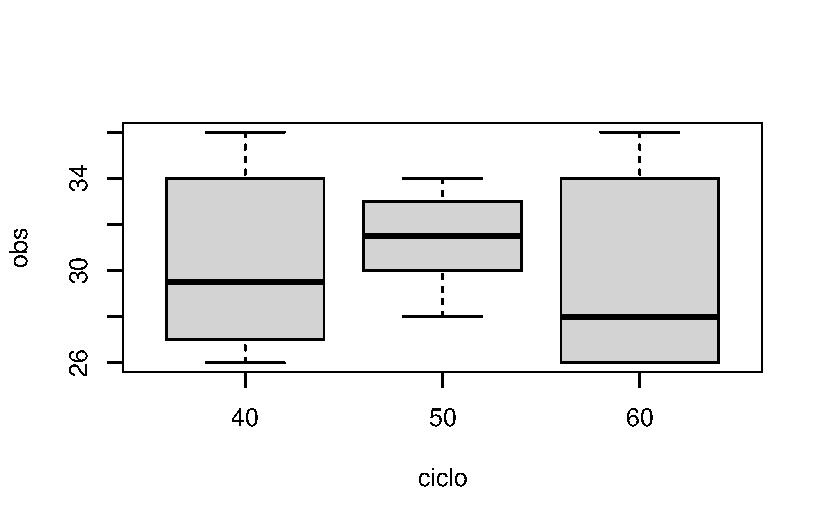
\includegraphics{fatorial_multi_files/figure-pdf/unnamed-chunk-3-1.pdf}

}

\end{figure}

\begin{Shaded}
\begin{Highlighting}[]
\FunctionTok{boxplot}\NormalTok{(obs}\SpecialCharTok{\textasciitilde{}}\NormalTok{oper)}
\end{Highlighting}
\end{Shaded}

\begin{figure}[H]

{\centering 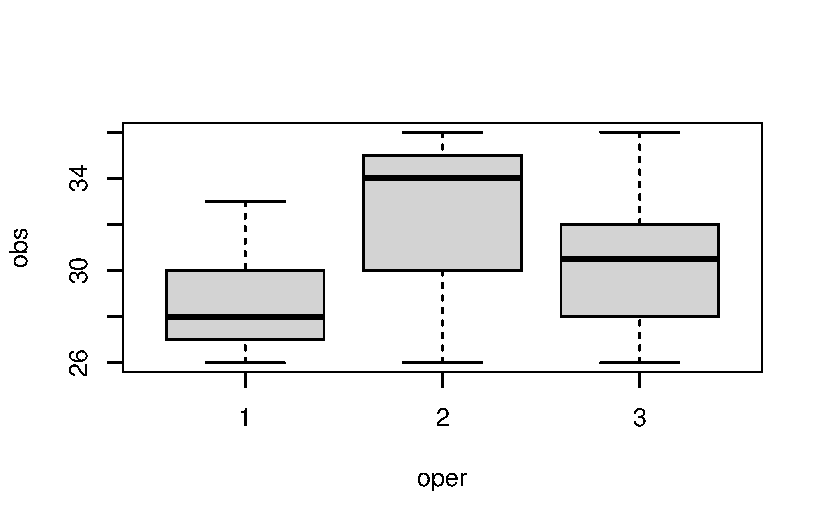
\includegraphics{fatorial_multi_files/figure-pdf/unnamed-chunk-3-2.pdf}

}

\end{figure}

\begin{Shaded}
\begin{Highlighting}[]
\FunctionTok{boxplot}\NormalTok{(obs}\SpecialCharTok{\textasciitilde{}}\NormalTok{temp)}
\end{Highlighting}
\end{Shaded}

\begin{figure}[H]

{\centering 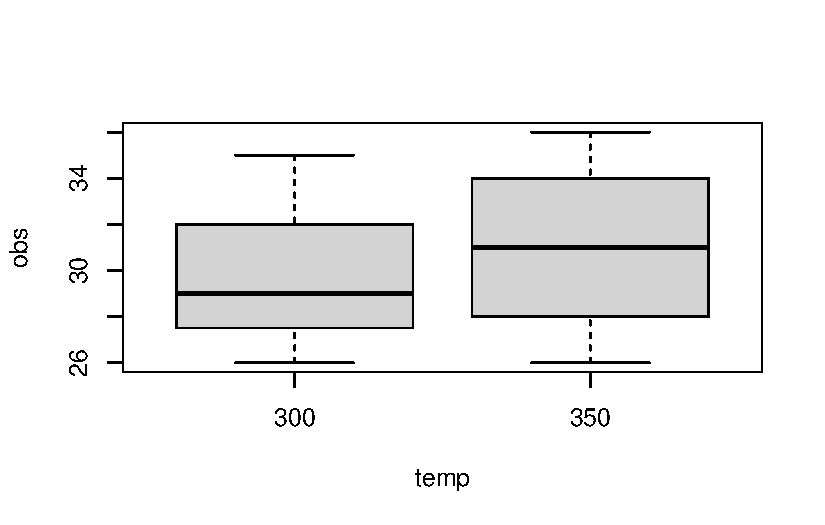
\includegraphics{fatorial_multi_files/figure-pdf/unnamed-chunk-3-3.pdf}

}

\end{figure}

\begin{Shaded}
\begin{Highlighting}[]
\FunctionTok{boxplot}\NormalTok{(obs}\SpecialCharTok{\textasciitilde{}}\NormalTok{ciclo}\SpecialCharTok{*}\NormalTok{oper}\SpecialCharTok{*}\NormalTok{temp)}
\end{Highlighting}
\end{Shaded}

\begin{figure}[H]

{\centering 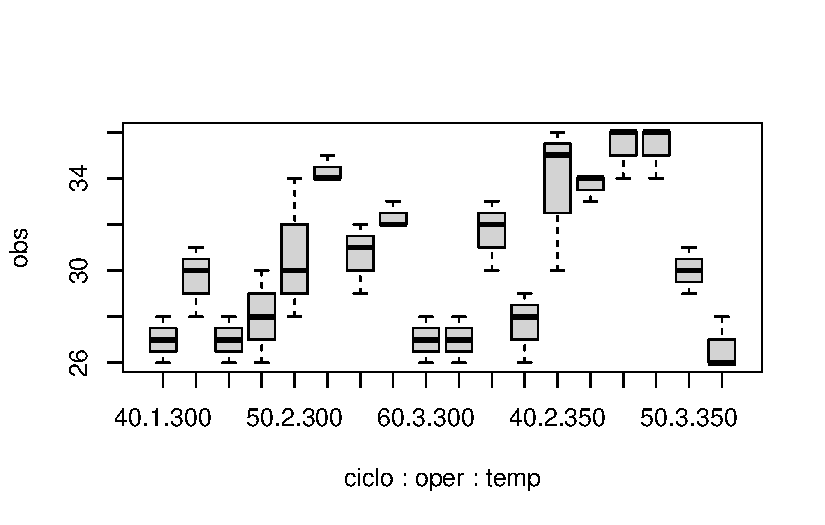
\includegraphics{fatorial_multi_files/figure-pdf/unnamed-chunk-3-4.pdf}

}

\end{figure}

\hypertarget{quais-suxe3o-as-hipuxf3teses-de-interesse}{%
\section{1.1 Quais são as hipóteses de
interesse?}\label{quais-suxe3o-as-hipuxf3teses-de-interesse}}

\hypertarget{do-estudo}{%
\subsection{Do estudo}\label{do-estudo}}

\[\begin{cases}
H_{0}: \mbox{Os fatores não apresentam efeitos no tecido} \\
H_{1}: \mbox{Os fatores apresentam efeitos no tecido}\\
\end{cases}\]

\hypertarget{do-modelo-de-anuxe1lise-fatorial}{%
\subsection{Do modelo de Análise
Fatorial}\label{do-modelo-de-anuxe1lise-fatorial}}

\[\begin{cases}
H_{0}: \mbox{$\tau_{1}= ... = \tau_{a} = 0} \\
H_{1}: \mbox{\tau_{i}!= 0}\\
\end{cases}\]

\[\begin{cases}
H_{0}: \mbox{\alpha_{1}= ... = \alpha_{a} = 0} \\
H_{1}: \mbox{\alpha_{i}!= 0}\\
\end{cases}\]

\[\begin{cases}
H_{0}: \mbox{\beta_{1}= ... = \beta_{a} = 0} \\
H_{1}: \mbox{\beta_{i}!= 0}\\
\end{cases}\]

\[\begin{cases}
H_{0}: \mbox{(\tau\beta)_{ij}= 0} \\
H_{1}: \mbox{(\tau\beta)_{ij}!= 0}\\
\end{cases}\]

\[\begin{cases}
H_{0}: \mbox{(\alpha\beta)_{ij}= 0} \\
H_{1}: \mbox{(\alpha\beta)_{ij}!= 0}\\
\end{cases}\]

\[\begin{cases}
H_{0}: \mbox{(\tau\alpha)_{ij}= 0} \\
H_{1}: \mbox{(\tau\alpha)_{ij}!= 0}\\
\end{cases}\]

\[\begin{cases}
H_{0}: \mbox{(\tau\beta\alpha)_{ij}= 0} \\
H_{1}: \mbox{(\tau\beta\alpha)_{ij}!= 0}\\
\end{cases}\]

\hypertarget{anuxe1lise-de-variuxe2ncias}{%
\section{1.2 Análise de Variâncias}\label{anuxe1lise-de-variuxe2ncias}}

\begin{Shaded}
\begin{Highlighting}[]
\NormalTok{anova }\OtherTok{\textless{}{-}} \FunctionTok{aov}\NormalTok{(obs}\SpecialCharTok{\textasciitilde{}}\NormalTok{ciclo}\SpecialCharTok{*}\NormalTok{oper}\SpecialCharTok{*}\NormalTok{temp)}
\FunctionTok{summary}\NormalTok{(anova)}
\end{Highlighting}
\end{Shaded}

\begin{verbatim}
                Df Sum Sq Mean Sq F value   Pr(>F)    
ciclo            2  25.59   12.80   5.357  0.00919 ** 
oper             2 164.93   82.46  34.519 4.26e-09 ***
temp             1  34.24   34.24  14.333  0.00056 ***
ciclo:oper       4 193.85   48.46  20.287 8.05e-09 ***
ciclo:temp       2  23.59   11.80   4.938  0.01273 *  
oper:temp        2  18.04    9.02   3.775  0.03248 *  
ciclo:oper:temp  4  34.96    8.74   3.659  0.01336 *  
Residuals       36  86.00    2.39                     
---
Signif. codes:  0 '***' 0.001 '**' 0.01 '*' 0.05 '.' 0.1 ' ' 1
\end{verbatim}

\hypertarget{conclusuxf5es}{%
\subsection{Conclusões}\label{conclusuxf5es}}

Com \(\alpha=5%
\), todas as \(H_{0}\) do modelo são rejeitadas, indicando que existem
diferenças.

\hypertarget{anuxe1lise-dos-pressupostos}{%
\section{1.3) Análise dos
pressupostos}\label{anuxe1lise-dos-pressupostos}}

Para o modelo de Análise Fatorial, os pressupostos são Normalidade,
Independência dos resíduos e Homocedasticidade.

\hypertarget{normalidade}{%
\subsection{Normalidade}\label{normalidade}}

\begin{Shaded}
\begin{Highlighting}[]
\FunctionTok{qqnorm}\NormalTok{(anova}\SpecialCharTok{$}\NormalTok{residuals)}
\FunctionTok{qqline}\NormalTok{(anova}\SpecialCharTok{$}\NormalTok{residuals)}
\end{Highlighting}
\end{Shaded}

\begin{figure}[H]

{\centering 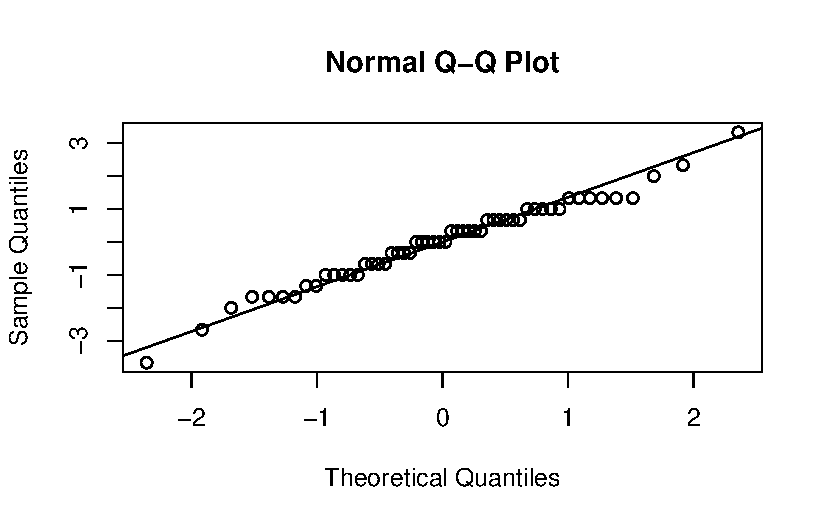
\includegraphics{fatorial_multi_files/figure-pdf/unnamed-chunk-5-1.pdf}

}

\end{figure}

\begin{Shaded}
\begin{Highlighting}[]
\FunctionTok{shapiro.test}\NormalTok{(anova}\SpecialCharTok{$}\NormalTok{residuals)}
\end{Highlighting}
\end{Shaded}

\begin{verbatim}

    Shapiro-Wilk normality test

data:  anova$residuals
W = 0.98124, p-value = 0.555
\end{verbatim}

\hypertarget{independencia}{%
\subsection{Independencia}\label{independencia}}

\begin{Shaded}
\begin{Highlighting}[]
\FunctionTok{plot}\NormalTok{(anova}\SpecialCharTok{$}\NormalTok{residuals)}
\end{Highlighting}
\end{Shaded}

\begin{figure}[H]

{\centering 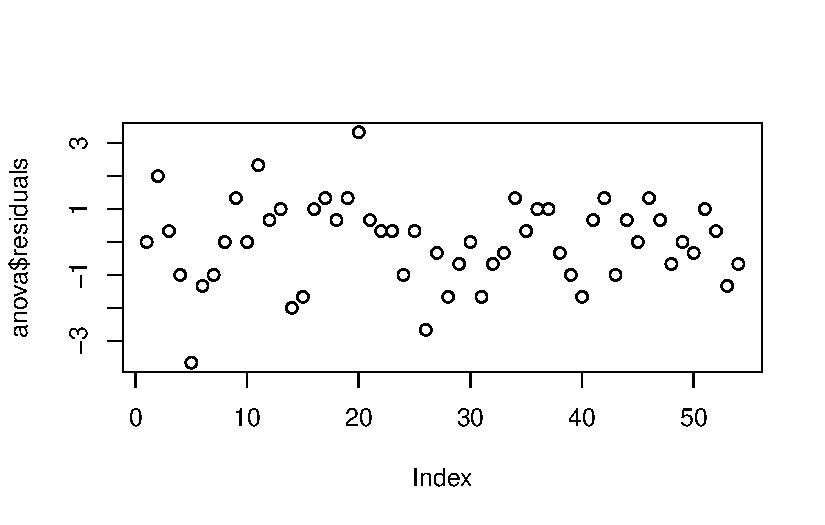
\includegraphics{fatorial_multi_files/figure-pdf/unnamed-chunk-6-1.pdf}

}

\end{figure}

\begin{Shaded}
\begin{Highlighting}[]
\FunctionTok{plot}\NormalTok{(anova}\SpecialCharTok{$}\NormalTok{residuals}\SpecialCharTok{/}\FunctionTok{summary}\NormalTok{(anova)[[}\DecValTok{1}\NormalTok{]][}\DecValTok{4}\NormalTok{,}\DecValTok{3}\NormalTok{])}
\end{Highlighting}
\end{Shaded}

\begin{figure}[H]

{\centering 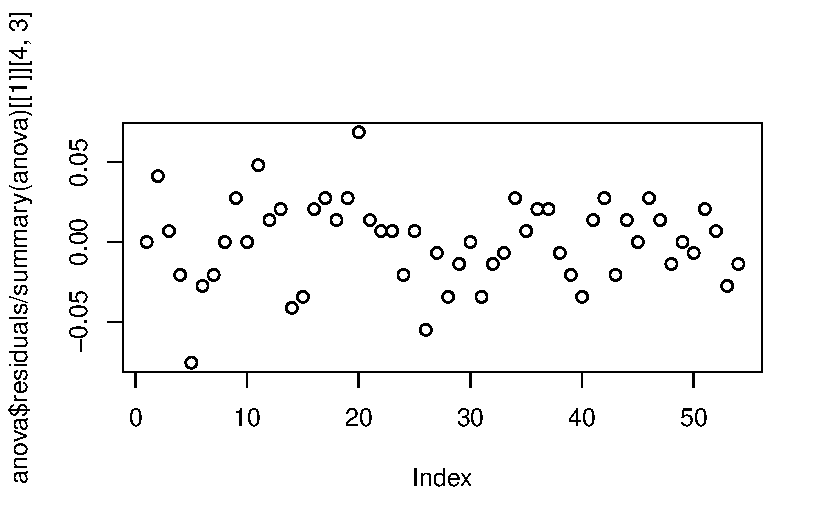
\includegraphics{fatorial_multi_files/figure-pdf/unnamed-chunk-6-2.pdf}

}

\end{figure}

\hypertarget{homocedasticidade}{%
\subsection{Homocedasticidade}\label{homocedasticidade}}

\begin{Shaded}
\begin{Highlighting}[]
\FunctionTok{plot}\NormalTok{(anova}\SpecialCharTok{$}\NormalTok{residuals, anova}\SpecialCharTok{$}\NormalTok{fitted.values)}
\end{Highlighting}
\end{Shaded}

\begin{figure}[H]

{\centering 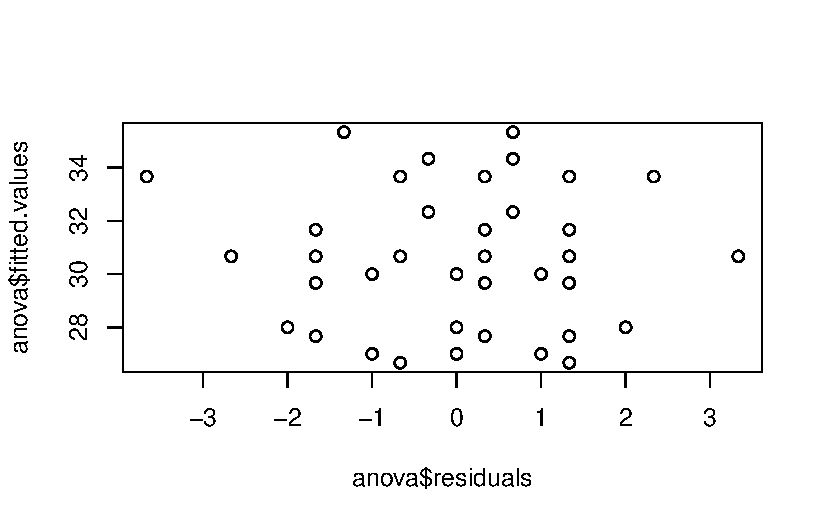
\includegraphics{fatorial_multi_files/figure-pdf/unnamed-chunk-7-1.pdf}

}

\end{figure}

\begin{Shaded}
\begin{Highlighting}[]
\FunctionTok{leveneTest}\NormalTok{(obs}\SpecialCharTok{\textasciitilde{}}\NormalTok{ciclo)}
\end{Highlighting}
\end{Shaded}

\begin{verbatim}
Levene's Test for Homogeneity of Variance (center = median)
      Df F value Pr(>F)
group  2  2.3955 0.1013
      51               
\end{verbatim}

\begin{Shaded}
\begin{Highlighting}[]
\FunctionTok{leveneTest}\NormalTok{(obs}\SpecialCharTok{\textasciitilde{}}\NormalTok{oper)}
\end{Highlighting}
\end{Shaded}

\begin{verbatim}
Levene's Test for Homogeneity of Variance (center = median)
      Df F value Pr(>F)
group  2  1.5477 0.2226
      51               
\end{verbatim}

\begin{Shaded}
\begin{Highlighting}[]
\FunctionTok{leveneTest}\NormalTok{(obs}\SpecialCharTok{\textasciitilde{}}\NormalTok{temp)}
\end{Highlighting}
\end{Shaded}

\begin{verbatim}
Levene's Test for Homogeneity of Variance (center = median)
      Df F value  Pr(>F)  
group  1  3.3024 0.07494 .
      52                  
---
Signif. codes:  0 '***' 0.001 '**' 0.01 '*' 0.05 '.' 0.1 ' ' 1
\end{verbatim}

\hypertarget{section}{%
\section{1.4)}\label{section}}

\hypertarget{h_0-rejeitada-e-auxed}{%
\subsection{\texorpdfstring{\(H_{0}\) rejeitada e
aí}{H\_\{0\} rejeitada e aí}}\label{h_0-rejeitada-e-auxed}}

\begin{itemize}
\tightlist
\item
  Como a pontuação média varia de acordo com os fatores?
\item
  Qual combinação maximiza a pontuação?
\end{itemize}

\begin{Shaded}
\begin{Highlighting}[]
\FunctionTok{TukeyHSD}\NormalTok{(anova, }\AttributeTok{which=}\StringTok{"ciclo"}\NormalTok{)}
\end{Highlighting}
\end{Shaded}

\begin{verbatim}
  Tukey multiple comparisons of means
    95% family-wise confidence level

Fit: aov(formula = obs ~ ciclo * oper * temp)

$ciclo
            diff        lwr        upr     p adj
50-40  1.0555556 -0.2037488  2.3148599 0.1152084
60-40 -0.6111111 -1.8704155  0.6481933 0.4689489
60-50 -1.6666667 -2.9259710 -0.4073623 0.0071848
\end{verbatim}

\begin{Shaded}
\begin{Highlighting}[]
\FunctionTok{interaction.ABC.plot}\NormalTok{(obs,ciclo, oper, temp, }\AttributeTok{data=}\NormalTok{df)}
\end{Highlighting}
\end{Shaded}

\begin{figure}[H]

{\centering 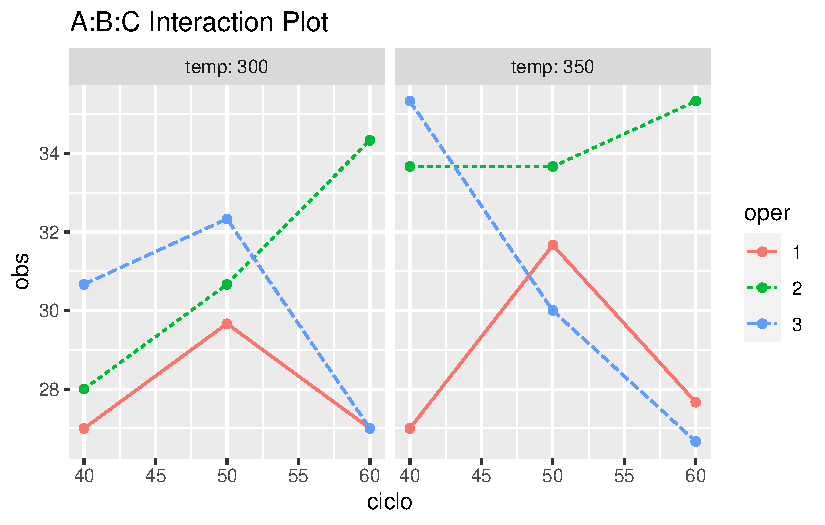
\includegraphics{fatorial_multi_files/figure-pdf/unnamed-chunk-8-1.pdf}

}

\end{figure}



\end{document}
